\section{Background}
\label{sec:basics}

In the following, a short overview on underlying technologies is given. 
\begin{figure}
  \centering
    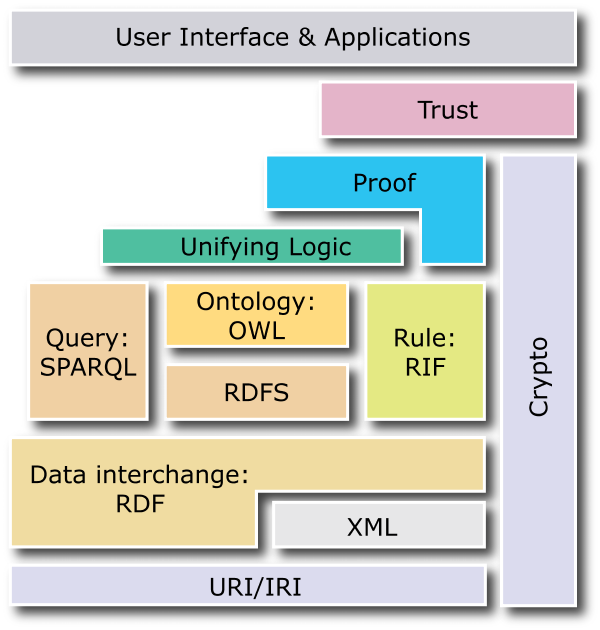
\includegraphics[width=0.5\textwidth]{layerCake.png}
  \caption{Semantic Web Technologien}
  \label{fig:layercake}
\end{figure}

\subsection{Semantic Web}
The world wide web is one the most important inventions of our time. 
It enables the global access to documents and real time communication between individuals.
This achieved by an interoperable infrastructure of independent networks, that can route any communication between two points.
From our current perspective on the last three decades, this even seems technologically simple and maintainable at a reasonable cost.
Furthermore the resulting benefits to our economy and society are beyond all expectations. A hole new industry was created and most industries are substantially influenced in their processes.
The costs of communications dropped and public and private communications alike switched mostly to the new medium.
The world wide web is enabled by a set of related technologies, which can be summarized to the following core concepts:
\begin{itemize}
\item TCP/IP addressing, transmission and routing
\item client/server communication protocols like HTTP
\item interlinked documents containing data (e.g. XML) or services (or interactive content) valuable for humans
\end{itemize}
While these technologies are well established and scale up to a huge amount of data, the users --- humans --- can barely cope with this amount of data offered. 
If one considers the WWW a information system, it only offers basic retrieval methods and most critical, it is fragmented into heterogeneous subsystems (which however can offer very good retrieval methods). 
But global interoperability is not supported on content level. 
Data is controlled by applications, and each application keeps it to itself\footnoteUrl{http://www.w3.org/2001/sw/}.
From a perspective of data integration, semantics are often vague or undefined. 
It is often unclear which entity a document refers to. 
Documents are only interlinked by untyped relations. 
These are strong limitations: if the data is too much for a human to read and machines do not have deeper insight into it, the dataset as a whole can be seen as inaccessible. 
Of course the way the WWW works today seems to be well suited. 
Programmable Webservers e.g. with PHP made the web interactive, enabling social interaction or collaborative editing. But still future development is blocked by the human-centric nature of the web. 
If all the knowledge humanity acquired and wrote down in e.g. Wikipedia would be also available to information systems in a structured way, even more knowledge could be inferred automatically and e.g. artificial intelligence, expert systems or search would be boosted dramatically. 
The key to solving this issue lies (according to \cite{berners}) in the establishment of \textit{Linked Data} (which will be explained in the next section). 
The use of machine readable data and annotation of text with such data is crucial for information technology to enter the next level.
So to conclude: the problem is the amount of knowledge, and the lack of formalization e.g. machine readability. 
Even data that is already structured often lacks a defined semantic or the semantic is not formalized. 
The web as we know it is a web of documents, the target is the web of data. 
Instead of just documents linking to each other, instances should be globally interlinked. 
Consider this example: A company stores costumer information about you in its relational database; facebook keeps record of your activities in their distributed database and you yourself have a blog on your own webserver. 
Why shouldn't all this personal information be linked\footnote{The reader may object privacy issues; but the focus of this thesis is on data integration. These two topic have to be considered separately: just because data is interoperable, it is not accessible. 
Even more: if you avoid redundancy, you gain control over your data. 
How this control can be achieved is topic to current research but already very promising. Cf. WebID}? By a global identifier for \textit{you}. 
Why do we have to supply contact information over and over again, although its database 101 that redundancy is bad. 
The answer is incompatibility on many levels. The ideal would be that all data is interoperable by design. 
Shortly after the invention of concepts for the WWW, Tim Berners-Lee et al. came up with the idea of the Semantic Web: an WWW where intelligent agents can act on behalf of users, to find information or communicate.
They have a shared syntax and vocabulary, use ontologies as background knowledge and thus get deeper to the intended semantic of things.
The Semantic Web (SW) is a set of complementary technologies, which are depicted in figure~\ref{fig:layercake}. 
It is a layered model to represent, query and manage information.\\
The effort was initiated in 2001 by Tim Berners-Lee, who defined it as 
\begin{quote}
"`an extension of the current web in which information is given well-defined
meaning, better enabling computers and people to work in cooperation"'.
\cite{berners}
\end{quote}
There are several ways to augment information for better machine readability: 
One is the annotation of old fashioned documents with well defined shared vocabularies. 
An example for annotations is RDFa\footnoteUrl{http://www.w3.org/TR/xhtml-rdfa-primer/}. 
It allows to add structured information to arbitrary HTML documents. 
The second way is the creation of stand alone ontologies: An ontology is a specification of a conceptualization \cite{gruber}.
A conceptualization refers to some model of the world, created by a subject, for some purpose, that is shared by a group of individuals.
\begin{quote}
A body of formally represented knowledge is based on a conceptualization: the objects, concepts, and other entities that are assumed to exist in some area of interest and the relationships that hold among them \cite{genesereth}. 
A conceptualization is an abstract, simplified view of the world that we wish to represent for some purpose. 
Every knowledge base, knowledge-based system, or knowledge-level agent is committed to some conceptualization, explicitly or implicitly. \cite{gruber}
\end{quote}
A specification refers to a formal notion of the conceptualized knowledge.
\begin{quote}
When the knowledge of a domain is represented in a declarative formalism, the set of objects that can be represented is called the universe of discourse. 
This set of objects, and the describable relationships among them, are reflected in the representational vocabulary with which a knowledge-based program represents knowledge. 
Thus, in the context of AI, we can describe the ontology of a program by defining a set of representational terms. 
In such an ontology, definitions associate the names of entities in the universe of discourse (e.g., classes, relations, functions, or other objects) with human-readable text describing what the names mean, and formal axioms that constrain the interpretation and well-formed use of these terms. 
[...]
Formally, an ontology is the statement of a logical theory. 
[...]
Ontologies are often equated with taxonomic hierarchies of classes, but class definitions, and the subsumption relation, but ontologies need not be limited to these forms.
[...]
In short, a commitment to a common ontology is a guarantee of consistency,
\cite{gruber}
\end{quote}

The usage of shared, formal ontologies (which implies the agreement on a vocabulary and hence a common \textit{language}) and the development of open standards shall provide provides contracts for agents that act on behalf of a information interest of humans. 
The reuse of existing webstandards (like URIs or the HTTP protocol) shall promote a fast adoption. 
The target is to make knowledge globally interoperable between different schemata and humans and machines alike. 
Therefore knowledge becomes usable for software systems which allows for pioneering usage scenarios (cf. \cite{hitzler}).\\

\subsection{RDF}
The central technology to enable these ideas is RDF\footnoteUrl{http://www.w3.org/RDF/}. 
RDF itself is a universal data model, that dictates how information may be medelled on a structural level. RDF/XML\footnoteUrl{http://www.w3.org/TR/rdf-syntax-grammar/} or  N3\footnoteUrl{www.w3.org/DesignIssues/Notation3} and others are serialization formats for RDF that are defined on syntactical level.
RDF is an acronym for Resource Description Framework. 
The basic idea is the identification of the \textit{things and relations} within the universe of discourse (not just websites), with an URI\footnoteUrl{http://tools.ietf.org/html/rfc3986}. 
About those resources, statements can be made in the form of \textit{"subject predicate object"} --- analogously to a natural language sentence. 
These statements are also called triples.\\
For example the triple 
\begin{lstlisting}[style=N3]
<http://example.com/Alice> rdf:type foaf:Person
\end{lstlisting}
encodes the fact that ``Alice is a person'' (if the vocabulary has been defined accordingly). 
Notice: subject, predicate and object are URIs, but the predicate uses the prefix \texttt{rdf}, which is an abbreviation for an actual URI. 
The definition of this prefix would be \verb+@PREFIX rdf: <http://www.w3.org/1999/02/22-rdf-syntax-ns#>+. 
The class \texttt{Person} has been taken from the foaf vocabulary\footnoteUrl{http://xmlns.com/foaf/0.1/}, which offers terms for people in a social environment. 
The triple can be interpreted as a directed graph: subject and object are nodes --- the predicate is a typed edge.\\
\begin{figure}[h]
  \centering
    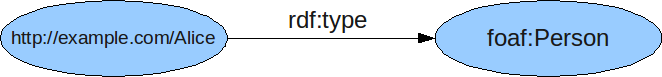
\includegraphics[width=0.5\textwidth]{triple-graph.png}
  \caption{The triple as a graph}
  \label{fig:triple-graph}
\end{figure}
\\
Multiple triples can be grouped in a graph, which is in turn identified by an URI. 
Such a graph can be used as an ontology. 
Thus ontologies in RDF format are actually graph databases which are inherently easily accessible for algorithms as opposed to natural language which always introduces ambiguity and noise. 
It is surprisingly easy to model even complex data or schemata in graphs. 
And additionally the formalized knowledge becomes easily accessible. 
Implicit information can be inferred (e.g. transitive relations or inherited properties) or contractions can be detected\footnote{Access Control, Logic and Proof: \url{http://www.w3.org/2000/01/sw/#access}}.\\
In contrast to tree based models like XML, a relation does not have to be allocated to one of the participating entities. 
This eliminates a frequent modelling dilemma. 
Futher more such a flat net equates more to the decentral nature of the web: The information is distributed and when merging two knowledge bases --- at least at this level --- there is no problem with schema normalization (cf. \cite{hitzler}). 
Of course there can be different schemas, but (according to the classification of heterogeneity in \cite{ouksel}) the problem can be reduced to its core --- semantic heterogeneity, but for example schematic heterogeneity as in relational systems or XML can be solved by design. 
Object matching can be avoided where possible or wanted, reusing vocabularies and URIs in the ontology creation process.\footnote{In practice the problem still persists due to administrative autonomy. 
Existing vocabularies are not reused due to lack of information, strategic decisions or suspected semantic mismatches. 
Schema and object matching in the semantic web is subject to ongoing research.}\\
To complete the introduction of RDF, it is necessary to present the notion of data values. For example the number 5 or the string "abc" are not assigned URIs. 
It would make no sense as they are no independent entites within the universe of discourse. 
They are the value of properties and so they are assigned the special node type  Literal\footnoteUrl{http://www.w3.org/TR/rdf-concepts/#section-Graph-Literal}. 
They can not be subject for further statements. 
There are three types of literals:
\begin{compactitem}
\item \textit{plain literals},
\item \textit{plain literals} with optional \textit{language tag} and 
\item \textit{typed literals}, that are augmented with a datatype, that is given by an URI.
\end{compactitem}
\vspace{0.2ex}
The NTriples serialization of a literal could be:

\begin{lstlisting}[style=N3]
ex:Alice foaf:birthday "22.09.1986"^^xsd:date
\end{lstlisting}
In the example a typed literal is used to represent a date. 
The XSD vocabulary\footnoteUrl{http://www.w3.org/2001/XMLSchema#} for basic datatypes is used.

RDF can be stored either in text files or with in special databases called \textit{triple stores}, where common database techniques like indexing, query languages or backups are possible. 
Some widely known triple stores are Virtuoso\footnoteUrl{http://virtuoso.openlinksw.com/dataspace/dav/wiki/Main/}, Sesame \footnoteUrl{http://www.openrdf.org/} or Jena\footnoteUrl{http://jena.apache.org/}. 
Storage backends vary widely from relational over graphs to in-memory.

\subsection{Linked Data}
\textit{Linked Data} is the simplest and yet most important mechanism to retrieve RDF data: as described, entities are identified by URI's. 
When choosing the URL's one should pick a namespace under her authority, so that she can provide \textit{some} data about that entity under that URL. As defined by W3C\footnoteUrl{http://www.w3.org/DesignIssues/LinkedData.html}, the requirements for Linked Data are as follows:

\begin{enumerate}
\item Use URIs as names for things
\item Use HTTP URIs so that people can look up those names
\item When someone looks up an URI, provide useful information, using RDF
\item Include links to other URIs, so that they can discover more things
\end{enumerate}
What is the rational behind doing so? 
\begin{quotation}
"The first \textit{Linked Data} principle advocates using URI references to identify, not just Web documents and digital content, but also real world objects and abstract concepts. 
These may include tangible things such as people, places and cars, or those that are more abstract, such as the relationship type of knowing somebody, the set of all green cars in the world, or the color green itself. 
This principle can be seen as extending the scope of the Web from online resources to encompass any object or concept in the world. 
The HTTP protocol is the Web’s universal access mechanism. 
In the classic Web, HTTP URIs are used to combine globally unique identification with a simple, well-understood retrieval mechanism. 
Thus, the second Linked Data principle advocates the use of HTTP URIs to identify objects and abstract concepts, enabling these URIs to be dereferenced (i.e., looked up) over the HTTP protocol into a description of the identified object or concept."~\cite{linkeddata-book}
\end{quotation}
The lookup of URI can even be enhanced with a mechanism called \textit{Content Negotiation}: Based on the HTTP \textit{accept} header (that is set by the application requesting), different types of formatting can be used in the response. 
If for example a human browses RDF data using a web browser, a HTML version of the RDF data can be generated easily. 
If an application requests RDF data it would set the accept header to \texttt{application/rdf+xml} and get XML, which easy to read by machines, nut not humans. The mechanism is also transparent, it happens server side at request time. 
Modern RDF stores like \textit{Virtuoso} have built in support for \textit{Linked Data} with \textit{Content Negotiation}.

These four basic principles together make a fundamental difference regarding the architecture of Linked Data seen as a database. 
Instead of custom communication protocols, well established web standards are used. 
This makes it interoperable at a technical level and easy to adopt.
And it is backward compatible to very simple solutions: If one wants to publish \textit{Linked Data}, no triple store is required at all, one could as well use a file server, with the documents available materialized.
Also \textit{Linked Data} implicitly is a \textit{basic distributed database}: Because the query language is limited to a simple GET (for now), one can easily distribute data on different physical servers, while having constant access costs. 
Also mirroring and load balancing is easy by deploying any default web proxy, because Linked Data integrates transparently with established web technologies. 
But besides these technical benefits, the most important is that linked data changes the way people administrate data. 
The integration aspect is being catered for by design and more important: the design also promotes data producers to regard integration issues at production time. 
If tool support grows fast enough, initial adoption costs and fears could be reduced. 
This would an overall decrease in integration efforts, which in turn would prosper knowledge intensive applications. 
As presented in the introduction, solving knowledge intensive problems will be one of the key challenges of the next decades.

To embed the technology centric RDF standard into general publishing decision (for example by governments), Tim Berners-Lee suggested a simple rating system regarding openness and interoperability:

  \begin{table}[htb]
  	\small
  	\caption{Five star rating of Linked Data}
	\begin{tabular}{rp{0.7\textwidth}}
$\bigstar$ & Available on the web (whatever format) (optionally with an open licence, to be \textit{Open Data}) \\ 
$\bigstar\,\bigstar$ & Available as machine-readable structured data (e.g. excel instead of image scan of a table) \\ 
$\bigstar\,\bigstar\,\bigstar$ &  two stars plus use of a non-proprietary format (e.g. CSV instead of excel) \\ 
$\bigstar\,\bigstar\,\bigstar\,\bigstar$ & All the above plus, Use open standards from W3C (RDF and SPARQL) to identify things, so that people can point at your stuff \\ 
$\bigstar\,\bigstar\,\bigstar\,\bigstar\,\bigstar$ & All the above, plus: Link your data to other people’s data to provide context
    \end{tabular}
  \end{table}
It gives data producers a roadmap to high quality data and consumers objective hint about published datasets.

\subsection{SPARQL} \label{sec:sparql}
How can one query RDF data in a more sophisticated way that just the retrieval of single resources? One may want to search data that matches certain constraints or access a full text index over the data.
SPARQL\footnote{\url{http://www.w3.org/TR/rdf-sparql-query/} \\
bzw. \url{http://www.dajobe.org/2005/04-sparql/SPARQLreference-1.8-us.pdf}} steht für \emph{SPARQL Protocol and RDF Query Language} und ist eine Anfragesprache für RDF-Graphen sowie ein Protokoll für deren Nutzung über einen Webservice. Mit ihr können Literale, Ressourcen oder ganze Teilgraphen extrahiert werden. Sie hat sich aus anderen Sprachen, wie SquishQL\footnote{siehe \cite{squishQL}}, RDQL\footnoteUrl{http://www.w3.org/Submission/RDQL/}, RQL\footnoteUrl{http://139.91.183.30:9090/RDF/RQL/} oder SeRQL\footnote{siehe \cite{serql}} (vgl. \cite{compQL}), entwickelt und stellt nun den offiziellen Standard des W3C dar.\\
Eine kurze Übersicht\footnote{Hier werden lediglich für das weitere Verständnis zentrale Ideen erläutert --- für eine umfassende und detaillierte Beschreibung ist der Standard zu konsultieren.} über die Features der Sprache werde ich im Folgenden geben.\\
\vspace{0.1cm}\\
Es gibt 4 Typen von SPARQL Querys:
\begin{itemize}
	\item{SELECT um Daten, die auf ein angegebenes Muster passen (\emph{matchen}), zu extrahieren}
	\item{ASK um zu prüfen, \emph{ob} ein Muster im Graph existiert}
	\item{CONSTRUCT gibt einen Graph zurück, der unter Umständen durch ein Such-Muster erzeugt wurde oder explizit angegeben wird}
	\item{DESCRIBE liefert Informationen über gematchte Ressourcen (ist nicht standardisiert, abhängig von der Konfiguration der Datenbank, oft beschreibende Eigenschaften, wenn diese eingetragen wurden)}
\end{itemize}
Eine SPARQL-Anfrage (Query) lässt sich in folgende Teile aufgliedern:
\begin{itemize}
	\item{Prolog\\um Prefixe und Base-URI zu deklarieren. 
	Relative URIs, die innerhalb des Querys vorkommen, werden auf die Base-URI bezogen. 
	Prefixe sind Abkürzungen für häufig verwendete URIs} 
	\item{Projektionsanweisung\\ähnlich SQL: Variablen (bei SQL Spalten), welche im Ergebnis sichtbar sein sollen oder "`*"' für alle verwendeten Variablen}
	\item{Ergebnis-Modifikatoren
	\begin{itemize}
		\item{DISTINCT zur Duplikatentfernung} 
		\item{REDUCED "`kann"' Duplikate entfernen, wenn dies für die Laufzeit sinnvoll ist.}
		\item{ORDER BY sorgt für Sortierung nach einem Ausdruck (oft einer Variablen)}
		\item{LIMIT und OFFSET um einen gewisses Intervall von Lösungen auszuwählen}
	\end{itemize}
	}
	\item{GraphPattern (und Construct Pattern bei CONSTRUCT Querys)\\
	geben einen Teilgraphen an und bestehen aus Tripeln oder weiteren GraphPattern, wobei allerdings Variablen genutzt werden können --- daher der Name Pattern. 
	Nach diesem Muster wird im Graph gesucht. 
	Mögliche Belegungen für Variablen sind das Ergebnis.
	Es gibt folgende GraphPattern-Typen:
	\begin{itemize}
		\item{GRAPH: ein elementares Pattern, bestehend aus einer beliebigen Folge von Tripeln, weiteren GraphPattern und Filtern. Ein Tripel ist eine Aussage aus dem angefragten RDF-Graph. Zwei aufeinanderfolgende Tripel werden durch einen Punkt getrennt und bilden eine Konjenktion dieser Aussagen. 
		Die Komponenten Subjekt, Prädikat und Objekt können durch Variablen ersetzt werden.}
		\item{OPTIONAL: ein GroupGraphPattern, das nicht notwendig ist. 
		Das heißt: Wenn dieses Teilmuster nicht gematcht werden kann, beinflusst dies nicht das matching des gesamten Musters --- allerdings sind enthaltene Variablen dann natürlich ungebunden.} 
		\item{UNION: verknüpft mehrere GraphPattern disjunktiv. 
		So können Alternativen ausgedrückt werden.}
	\end{itemize}
	\item{Filter sind logische Ausdrücke, die für jede mögliche Lösung\footnote{Eine Lösung ist eine Kombination von Variablen-Bindings, für die das Pattern \emph{matcht}.} evaluiert werden und (wenn sie zu \emph{false} ausgewertet werden) Ergebnisse löschen können. 
	Für die Ausdrücke steht eine logische, numerische und relative Algebra zur Verfügung, die über eingebaute und entfernte Funktionsaufrufe erweitert wurde.
	}
	}
\end{itemize}
Ein Beispiel Query:
\begin{lstlisting}[style=sparql]
PREFIX rdf: <http://www.w3.org/1999/02/22-rdf-syntax-ns#>
PREFIX foaf: <http://xmlns.com/foaf/0.1/>
SELECT ?subj ?name
WHERE {
    ?subj rdf:type foaf:Person .
    ?subj foaf:age ?age
    OPTIONAL { ?subj foaf:name ?name }
    FILTER( ?age > 23 )
}
\end{lstlisting}
Diese Anfrage findet alle Personen, die älter als 23 sind, und, wenn möglich, deren Namen. Genauer wird folgendes ausgedrückt: Zuerst wird ein Prefix deklariert, das das RDF und FOAF Vokabular abkürzt. 
Im WHERE-Teil wird ein GraphPattern angegeben, mit dem die Variable \texttt{?subj} mit allen Ressourcen belegt wird, für die die Aussage gilt, dass sie vom Typ \texttt{Person} aus dem FOAF-Vokabular sind. 
In der siebenten Zeile wird optional der zugehörige Name an die Variable \texttt{?name} gebunden. 
In der sechsten und achten Zeile wird abschließend noch eine Einschränkung auf das Alter deklariert, indem zunächst der Wert an eine Variable gebunden wird und diese dann mithilfe eines Filter-Ausdrucks eingeschränkt. 
Bei der Auswertung dieser Anfrage wird der sogenannte Triple-Store (also eine auf RDF-Daten spezialisierte Datenbank) versuchen, dieses Muster im angefragten Graph zu finden und alle möglichen Variablen-Belegungen als Ergebnis zurückliefern --- also beispielsweise eine Tabelle oder XML mittels eines speziellen Result-Set-Formats\footnoteUrl{http://www.w3.org/TR/rdf-sparql-XMLres/}.\\
\\

\subsection{Scenarios}
Now that we introduced many basics of the semantic web, one may ask: \textit{"What is it all good for? Why cant we solve this with traditional approaches?"}

Consider this example: Alice works as a journalist. She often has to research specific fields of history or science --- fields she is no expert in --- to support her articles. One day she has the information need for \textit{"Olympia winners before 1972 from countries with less than 10 million inhabitants"}. How long will it take her? A few hours maybe. Then her boss comes and asks her to change that search to \textit{"Olympia winners whose height is 10\% above their countries average, who were born on Mondays"}. This may  make no sense or her boss may be a maniac, but apparently the information is available somewhere in the internet --- most probably even in Wikipedia alone. And one could find it --- but it would take ages. Except if this information would be available in RDF. Then it would be seconds. This example should show that the computational access to information enables a vast amount of new knowledge that was hidden inside existing data.

Two problems come into play when trying to solve this scenario, which is an example for the research area of \textit{question answering}:

\begin{enumerate}
\item understanding the question
\item finding the answer
\end{enumerate}

The first could be solved by formalizing the question into a SPARQL query (by some black box of natural language processing magic), step 2 would require the information present in Wikipedia to be available in RDF.

The solution of the first one could be even assisted by the outcome of this thesis, as it provides for a large language resource, that can disambiguate query terms. The second one is tackled by a related (and yet larger and more important) project, which is presented in the next section.


\subsection{DBpedia}
To describe the Wikipedia and DBpedia project, I found it is highly sufficient to simply quote from each of their self-portrayals:
\begin{quote}
"Wikipedia is a free, collaboratively edited, and multilingual Internet encyclopedia supported by the non-profit Wikimedia Foundation. Its 22 million articles (over 4 million in English alone) have been written collaboratively by volunteers around the world. Almost all of its articles can be edited by anyone with access to the site, and it has about 100,000 regularly active contributors. As of August 2012, there are editions of Wikipedia in 285 languages. It has become the largest and most popular general reference work on the Internet, ranking sixth globally among all websites on Alexa and having an estimated 365 million readers worldwide. It is estimated that Wikipedia receives 2.7 billion monthly pageviews from the United States alone."\footnoteUrl{http://en.wikipedia.org/wiki/Wikipedia}
\end{quote}
DBpedia in turn wants to exploit this rich but unstructured dataset:
\begin{quote}
"The DBpedia project is a community effort to extract structured information
from Wikipedia and to make this information accessible on the Web. The resulting
DBpedia knowledge base currently describes over 2.6 million entities. For each of
these entities, DBpedia defines a globally unique identifier that can be dereferenced
over the Web into a rich RDF description of the entity, including human-readable
definitions in 30 languages, relationships to other resources, classifications in four
concept hierarchies, various facts as well as data-level links to other Web data
sources describing the entity. Over the last year, an increasing number of data
publishers have begun to set data-level links to DBpedia resources, making DBpedia
a central interlinking hub for the emerging Web of data. Currently, the Web of
interlinked data sources around DBpedia provides approximately 4.7 billion pieces of
information and covers domains such as geographic information, people, companies,
films, music, genes, drugs, books, and scientific publications." \cite{dbpedia_jws_09}
\end{quote}

"DBpedia allows you to ask sophisticated queries against datasets derived from Wikipedia and to link other datasets on the Web to Wikipedia data.
"\cite{dbpedia_iswc}
DBpedia is one of the most successful semantic web projects and has become a central linking hub of Linked Data.

\subsection{Related Work}\label{relatedWork}
%\subsection{Comparison of Wiktionary extraction approaches}
In the last five years, the importance of \wik as a lexical-semantic resource has been examined by multiple studies.
Meyer et al. (\cite{Meyer_2010a,Meyer_2010b}) presented an impressive overview on the importance and richness of \wik. 
In \cite{Zesch_2008_jwktl} the authors presented the \emph{JWKTL} framework to access \wik dumps via a Java API.
In \cite{meyer_2011b} this JWKTL framework was used to construct an upper ontology called \emph{OntoWiktionary}.
The framework is reused within the \emph{UBY project}~\cite{Gurevych_2012}, an effort to integrate multiple lexical resources (besides \wik also \emph{WordNet}, \emph{GermaNet}, \emph{OmegaWiki}, \emph{FrameNet}, \emph{VerbNet} and \emph{Wikipedia}).
The resulting dataset is modelled according to the \emph{LMF ISO standard}\cite{iso_24613-2008}.
\cite{Moerth_2011} and \cite{Declerck-2012} discussed the use of \wik to canonicalize annotations on cultural heritage texts (namely the Thompson Motif-index). 
Zesch et. al. also showed, that \wik is suitable for calculating semantic relatedness and synonym detection; and it outperforms classic approaches~\cite{Zesch_2008,Weale_2009}. 
Furthermore, other NLP tasks such as sentiment analysis have been conducted with the help of \wik \cite{Chesley_2006}.\\
Several questions arise, when evaluating the above approaches:
Why are there not more NLP tools reusing the free \wik data?
Why are there no web mashups of the data\footnote{For example in an online dictionary from \url{http://en.wikipedia.org/wiki/List_of_online_dictionaries}}?
Why has \wik not become the central linking hub of lexical-semantic resources, yet?\\
From our point of view, the answer lies in the fact, that although the above papers presented various desirable properties and many use cases, they did not solve the underlying knowledge extraction and data integration task sufficiently in terms of coverage, precision and flexibility.
Each of the approaches presented in Table \ref{tab:sota} relies on tools to extract machine-readable data in the first place.
In our opinion these tools should  be seen independent from their respective usage and it is not our intention to comment on the scientific projects built upon them in any way here. 
We will show the state of the art and which open questions they raise. 

\begin{table}[tb]
	\begin{tabular}{l|l|l|l|l|l|l}
        \centering
        % heading
		\textbf{name} & \textbf{active} & \textbf{available} & \textbf{RDF} & \textbf{\#triples} & \textbf{ld} & \textbf{languages}\\ \hline 
        % rows
JWKTL& \tickYes & dumps & \tickNo & - & \tickNo & en, de\\ 
wikokit & \tickYes & source + dumps &  \tickYes & n/a &\tickNo & en, ru\\ 
texai& \tickNo & dumps & \tickYes & $\sim$ 2.7 million & \tickNo & en\\ 
%\footnote{See \url{http://monnetproject.deri.ie/lemonsource/} and \cite{McCrae_2012}. The Wiktionary extraction tool is just a little sub project.} 
lemon scraper & \tickYes & dumps & \tickYes &$\sim$16k per lang& \tickNo & 6\\ 
blexisma& \tickNo & source & \tickNo & - & \tickNo & en\\ 
WISIGOTH & \tickNo & dumps & \tickNo & - & \tickNo & en, fr\\ 
lexvo.org& \tickYes & dumps & \tickYes & $\sim$353k & \tickYes & en\\ 
	\end{tabular}
    \caption{Comparison of existing Wiktionary approaches (ld = linked data hosting). None of the above include any crowd-sourcing approaches for data extraction. The wikokit dump is not in RDF.}
		\label{tab:sota}
\end{table}
\textit{JWKTL} is used as data backend of \textit{OntoWiktionary} as well as  UBY\footnote{\url{http://www.ukp.tu-darmstadt.de/data/lexical-resources/uby/}, \url{http://www.ukp.tu-darmstadt.de/data/lexical-resources/uby/}} and features a modular architecture, which allows the easy addition of new extractors (for example \textit{wikokit}~\cite{wikokit} is incorporated).
The Java binaries and the data dumps in LMF are publicly available.
Among other things, the dump also contains a mapping from concepts to lexicalizations as well as properties for part of speech, definitions, synonyms and subsumption relations. 
The available languages are English, German (both natively) and Russian (through \textit{wikokit}).
According to our judgement, \textit{JWKTL} can be considered the most mature approach regarding software architecture and coverage and is the current state of the art. 
\textit{Texai}\footnoteUrl{http://sourceforge.net/projects/texai/} and \textit{Blexisma}\footnoteUrl{http://blexisma.ligforge.imag.fr/index.html} are also Java based APIs, but are not maintained anymore and were most probably made obsolete by changes to the \wik layout since 2009.
There is no documentation available regarding scope or intended granularity. 
A very fine grained extraction was conducted using WISIGOTH~\cite{sajous_2010}, but unfortunately there are no sources available and the project is unmaintained since 2010. 
Two newer approaches are the \textit{lexvo.org} service and the algorithm presented in \cite{McCrae_2012}.
The \textit{lexvo.org} service offers a linked data representation of \wik with a limited granularity, namely it does not disambiguate on sense level. 
The source code is not available and only the English \wik is parsed.
As part of the Monnet project\footnote{See \url{http://www.monnet-project.eu/}. A list of the adopted languages and dump files can be found at \url{http://monnetproject.deri.ie/lemonsource/Special:PublicLexica}}, McCrae et al.~\cite{McCrae_2012} presented a simple scraper to transform \wik to the \lemon RDF model~ \cite{lemon-eswc}.
The algorithm (like many others) makes assumptions about the used page schema and omits details about solving common difficulties (as shown in the next section). 
At the point of writing, the sources are not available, but they are expected to be published in the future. 
Although this approach appears to be the state of the art regarding RDF modelling and linking, the described algorithm will \textit{not scale to the community-driven heterogeneity} as to be defined in Section \ref{sec:problem}.
All in all, there exist various tools that implement extraction approaches at various levels of granularity or output format. 
In the next section, we will show several challenges that in our opinion are insufficiently tackled by the presented approaches. 
Note that this claim is not meant to diminish the contribution of the other approaches as they were mostly created for solving a single research challenge instead of aiming to establish \wik as a stable point of reference in computational linguistics using linked data.
\newpage
